\chapter{Solution}
\label{solution}
\lettrine[lraise=0.1, nindent=0em, slope=-.5em]{\color{Violet}T}{he} Solution chapter is divided int three phases. First, the design phase for planning on learning process. Second, development phase where authoring of learning material being held. Third, the implementation phase the piloting of the course, where each course are run-through with particular students/trainers to get feedback about timing, content and evaluation.



 
\section{Design and Planning of learning process}
The Design phase contains four steps: First, Design learning objectives. Second, design assessments for each objective. Third, choose a course format. Fourth, create an instructional strategy. \citep{website:design_phase_ADDIE}


\subsection{Design of the course content and learning objectives}

In analysis phase the learning outcomes were established. However to design assessments tests and learning material more detailed learning objectives are needed. Therefore each learning outcome are divided into smaller units.

For design an adequate course content two aspects are required, learning objectives and assessment tests. Likewise in software development field the tests should be designed first to ensure creation of consistent learning materials and labs. Therefore all learning objectives are given with evaluation methods and values.  

The terms and vocabulary used in assessment should stay on level the students should know at the end of the lab and derived from learning objectives established in analysis phase.

Because big amount of learning materials, tests and labs only some examples are included into Appendices as Preliminary Tests~\ref{Preliminary Tests}, Preliminary Course~\ref{Preliminary course - dpkg based GNU/Linux}, Protecting Web Application -- \ref{Protecting Web Application Against (D)DOS Attacks},~\ref{Protecting an Insecure Web Application}. However, other materials can be found on course syllabus page composed on section~\ref{Course Syllabus}.


\subsubsection{Pre-requirements courses}

During the analysis of the target group the need for preliminary course was decided to homogenize a knowledge and a skill level of the participants.

The objectives and assessments for preliminary course:
\begin{itemize}
\item Student are able to work in command line using GNU/Linux as working with files, manage software, manage disks and partitions, manage users and groups, configure networks and user login session. Minimal level for pass is to gain more then 50\% one of the tests included in Appendix~\ref{Preliminary Tests} in Table~\ref{tab:preliminary_practical_test}
\item Student are able to explain basic terminology of operating systems (Kernel, GUI, shell, Virtual Memory, Authentication, Authorization, RAM, Cache, puffer, latency, throughput, file system, process, thread, password hash, DAC, MAC, RBAC, command parameter, command flag, file system hierarchy, environment variable). Minimal level to pass is gather more then 51\% of closed book test like in sample in Appendix~\ref{Preliminary Tests}
\item Student are able to configure network in GNU/Linux and explain terms like gateway, netmask, IP address, port, IP alias, DNS servers. Minimal level to pass is configuring network for lab machines.
\item Student is able to read/modify and create simpler BASH, Python and PowerShell scripts. Minimal level of pass is create script with all common language construction in one particular language. Powershell scripting is included because furtherer labs contains also integration labs with Active Directory, SAMBA4, GNU/Linux servers and workstations and Windows workstations.
\end{itemize}

According to previous objectives six practical classes are needed:\footnote{All times are given in academic hours or days which equal 8 academic hours.}
\begin{enumerate}[label=LAB \arabic*.,leftmargin=*]
\item Operating system basics (one day)
\item Basic networking IPv4/IPv6, TCP/IP (one day)
\item GNU/Linux basics (and OpenBSD/FreeBSD basics) (16h) as describbed in Appendix~\ref{Preliminary course - dpkg based GNU/Linux} on page~\pageref{Preliminary course - dpkg based GNU/Linux}
\item Scripting in BASH (2 days)
\item Scripting in Python (1.5 days)
\item Scripting in PowerShell (1.5 days)
\end{enumerate}

\subsubsection{Root Services}
In this particular case term root services are described as \gls{NTP}, \gls{DNS}, \gls{DHCP} service.
After finishing this block student are able to configure root services and use those services in furtherer labs.
The objectives and assessments for Root Services lab:
\begin{itemize}
\item After finishing this lab student is able to install \gls{NTP} service on server and on client computer and configure client to use internal server (pool) and server to use upstream \gls{NTP} service and fall-back services. Minimal level to pass: Services are configured, and student demonstrates debug skills with different tools and user explains basic terms and (pool, stratum, delay , offset, jitter, drift)
\item After finishing this lab student is able to install \gls{DNS} service and configure clients for new server. Minimally, students are able to configure zones, reverse zones, master -- slave replica, forwarding, different type of records (like MX, A, CNAME, TXT for SPF, PTR) and use basic management utilities to reload zone, flush name, flush cache, add records dynamically, freeze and thaw zones). Configured service does recursive quires for one particular subnet and student are able to explain what DNS attacks are used and what is Open Resolver. Student tests \gls{EITC} nameserver and explains what is wrong with that.
\item After finishing this lab student is able to install \gls{DHCP} server and configure hosts using this service. Minimal level for pass: Student installs and configures service what gives networking configuration to client machine from range or using hardware address. Service updates \gls{DNS} records using shared key (Mandatory Access Control must not disabled for pass)
\end{itemize}
\begin{enumerate}[label=LAB \arabic*.,leftmargin=*]
  	\item NTP (4h)
  	\item DNS (2.5 days)
  	\item DHCP (one day)
\end{enumerate}

\subsubsection{Web and File services}
Configuring and securing web servers is essential skill required from system administrators. Therefore, web server installation, configuration and hardening are covered with this block. Because instructional goals and learning outcomes also require covering file services topic.

The objectives and assessments for Web and File services:

\begin{enumerate}
   \item Web server basics - installation of apache2 web server
  	\item Web server security - Protecting Web Application Against
(D)DOS Attacks
  	\item Web server security - securing vulnerable web application using application firewalls (3 days)
  	\item Fileserver (Samba3 and Samba4) (0.5 day)
\end{enumerate}


\subsection{Choosing course format}

e-learning format. Võib kasutada ka probleemipõhist õpet, koostööl põhinevat õpet, kogukonnal põhivevat õpet.

Choosing a course format is a delivery system like medium used to present the course.
- classroom
- e-course
- blended -combines different methods
- 




Two possible e-learning processes are common the self-paced and facilitated/instructor-led \citep[p.~10]{food2011learning}.

Do we use collaboration in learning? 

Do we use  e-tutoring, e-coaching, e-mentoring?

Do we use chronological order or problem based? (one is good for lecturing other for practical classes) Also possible ways is spiral order logical order etc {\color{red} (viidata) }

Is the content sufficient to gain learning outcomes?



\subsection{Instructional strategy}
Instructional strategy for course focuses of guaranteeing learning outcomes by motivation students using proper content and activities planning.


\subsubsection{Pre-instructional activities}
The main goal of pre-instructional activities is motivate the students by explaining to the students why topic started must be covered and what student will be able to do after practical class. Thereafter, present learning objectives and assessment requirements and pre-requirements for the class. However, the minimal requirement level are presented and some students are interested for higher challenges for them extra quests, exercisers are presented as-well.


\subsubsection{Content Presentation}
Most today’s students are bored when receiving only theoretical lecture. For example, 1/2 of students do not have sufficient knowledge to fully understood the topic, and 1/4 of the students know already the aspects given and only 1/4 of the students are in the suitable level.  However, the exact numbers varies but is possible, that similar situation occurs often. Therefore, practical classes and lectures are combined and all taking place in computer classes. Every student should take 15-30 minute long theoretical block followed with practical activities. In case of e-learning students can browse video recordings and do their labs where suitable for them.

\subsubsection{Learner's feedback and assessment}
After every class, lecture should gather feedback about objectives, theoretical parts, labs and assessments because the course is very intensive and when more then 1/3 students can not follow due some problems then next block will fail for those students because they are linked by topic.
Is also possible that for valuable feedback are sufficient to ask from students how they feel about the course.

\subsubsection{Follow-through activities}
For explaining some situation the active discussions are needed (possible discussion topics are shown in lab materials as questions for the students) as seen in lab material highlighted with blue box with caption Discussion:
\begin{Verbatim}[frame=single,
label=Discussion,framesep=2mm,rulecolor=\color{blue},commandchars=\\\{\}]
Why You can not login into server?
Look at the server console. What is the OOM? What is the OOM killer?
\end{Verbatim}
In case of distance study and self study the discussions should being held using course Skype list. For conclude the discussion the lecturer must give feedback for each discussion topic using same channel or course e-mail list (In \gls{EITC} lecturer can send e-mail messages to all students participating this particular course).



\subsection{Pedagogical view of the e-course}
Different Pedagogical strategies can be used during learning process. First a problem based approach is {\color{red} Pooleli }
Second koostööl põhinev õpe ja kolmas kogukonnal põhinev õpe.

Do we use group-work, wiki, blog and/or some e-learning environment?

Synchronous or asynchronous learning.

\subsection{Planning grading/assessment techniques}
What grading methods are useful for this particular course?

Do we need grade knowledge, skills and {\color{red} Pooleli }

Several assessment methods are used to give feedback and grades for students in e-courses {\color{red} Viide+listile viide }

\begin{itemize}
	\item self-assessment
	\item computer assessment
	\item tutor assessment
	\item peer assessment
\end{itemize}
\subsection{Choosing technological tools}
For choosing technological tools for a course several following aspects need to be considered:

\begin{itemize}
	\item Availability of e-learning course
	\item usability of e-learning course
	\item Support for peer assessment and community based learning
	\item Support for realistic environment (more then one virtual machine for most of the labs)
	\item Standard complacence
\end{itemize}

For maintaining course materials, collaborations between students and lectures several Learning Management System (\gls{LMS}) are used by Estonian higher educational institutes. Incomplete list  of \gls{LMS}'s are Moodle, Blackboard WebCT (retried), CISO Network Academy, IVA, Sakai and Wikiversity. However the \gls{LMS} are useful for collaboration and storing learning material they can not be used as primary platform for new e-learning course because some grave limitations as: Firstly, the laboratories need virtual machines with administrative privileges in some cases  and supportive infrastructure to simulate Internet around the server. Secondly, only wikiversity and other wiki based systems are suitable for community based learning and peer assessment where students can teach and give feedback to others. Therefore no special \gls{LMS} are used in this course and materials are published in wiki, or in course web page. 






Õpiväljundid on mõeldud õppijate jaoks, et anda neile ülevaade sellest, mida kursuselt oodata ning
millele selle jooksul rõhku panna. Sellest lähtuvalt tuleks nad ka sõnastada vastavalt, st mitte õpetaja
vaid just õppijakeskselt, kirjeldades mitte seda, mis toimub kursuse käigus vaid keskendudes sellele,
mida uut peaks õppija suutma teha kursuse lõpuks.

\begin{enumerate}[label=Learning Objective \arabic*.,leftmargin=*]
\item NTP, DNS ,DHCP
\item Web server, OWASP, DVWA,
\item VPN, SAN, NAS, IDS, IPS
\end{enumerate}

\url{http://blog.spiderlabs.com/2011/01/detecting-malice-with-modsecurity-csrf-attacks.html}



\begin{enumerate}
\item Create a Sample (see on kliendile, testiks ja prototüübiks)
\item Develop the course Materials (peab teadma activities + tagasiside review)
\item Conduct a Run-through (real-time rehearsal testi sõbra peal kogu kursust +  feedback assessment + saab reaalselt teada aja, mis kulub kursuse läbimisele
\end{enumerate}


The implementation phase of the ADDIE Model contains three sub-phases

\begin{enumerate}
\item Train the Instructor
\item Prepare the Learners
\item Arrange the Learning Space
\end{enumerate}

Train the Instructor - course developer is often a trainer too but some cases you need more people to train


Development:
Authoring
Media creation / integration / production
Prototyping
Processing
Quality Assurance

\section{Development of the e-learning course}
The Development phase  (create a sample instruction and evaluate, create course materials - and review, conduct a run-through (a real-time rehearsal of the course) saab tagasisidet ja teada aja, mis on vaja kursuse läbimiseks)

\subsection{Authoring the learning material}
Developing learning material is based on learning objectives. Each learning objective must be covered with learning material and everything else should left out as extra load for student. Therefore in the development phase the authoring of different study materials, assessment tests, audio/video media and integration of all artefacts into consistent body with one reason: ensure that all objectives are met.

Authoring the study materials is one of most time consuming tasks and amount of developed study materials is too big even for appendices. Therefore one sample block - Securing web applications are included in Appendix~\ref{Protecting Web Application Against (D)DOS Attacks} and in Appendix~ \ref{Protecting an Insecure Web Application} 

Developed learning material are publicly available and under (\gls{CC-BY-SA}) license to guarantee maximum impact on field. Therefore is acceptable that people with will and motivation may self-study using this e-learning course. Moreover, the private training companies can use those courses to train target group.

Learning materials, self-tests, course information and other materials are publicly downloadable \footnote{\href{http://elab.itcollege.ee:8000/cyber-course/}{Course Syllabus (Õpijuhis)}}.


Some never materials are developed using open source revision control system \gls{git} and all changes and commits are publicly available. Moreover, source code of this thesis and labs are available from public \gls{git} repository with \LaTeX  source files and as well other files \footnote{\href{https://github.com/magavdraakon/margus-thesis.git}{Materials and source code of this thesis}}.





\url{http://www.grayharriman.com/ADDIE.htm}

Developed learning material should follow consistent style and present also one example of good documentation practice. For system administrators several howto styles exists. However practical hands-on laboratory instructions are designed that pass through using copy paste is possible but gives one working sample. However, this is not enough to pass lab scenario and student must customize own configuration.

Guiding stile of the lab instruction using style convention: First, all variable parts of the text are clearly differs from other text and command. Second, all commands given by student are highlighted, and variable parts embossed as seen in followed command.


\begin{minted}[frame=lines,framesep=2mm]{bash}
#For changing Out of memory - OOM adjustment score for mysql server
echo "-1000" > /proc/$(pidof mysqld)/oom_score_adj
\end{minted}
%$



Sample sample: Finding a proccess ID of the mysql server proccess.

\begin{minted}[frame=lines,framesep=2mm]{bash}
ps -ef|grep mysqld
\end{minted}
\label{code_sample}
%
\small{
\begin{Verbatim}[frame=single,
label=Command output,framesep=2mm,rulecolor=\color{red},commandchars=\\\{\}]
sudent@opiise:~# ps -ef|grep mysqld
root     11290 10905  0 10:27 pts/6    00:00:00 grep --color=auto mysqld
mysql    \fbox{\color{red}29830}    1  0 Apr25 ?        00:05:47 /usr/sbin/mysqld
\end{Verbatim}
%
}

All study should stored in open formats, like pdf, OpenDocument , MediaWiki markup language, html, utf8 text. Original editable source files for generating pdf, images should be publicly accessible. Moreover, text based materials should stored into version control system like \gls{git} to enable contributing for other lecturers and students as well.



\begin{table}[H]
\centering
\caption{The learning materials}

\begin{tabular}{|p{5cm}|p{3cm}|p{6cm}|}
\hline 
\color{blue}
Name & \color{blue} Comments  & \color{blue} Location \\ 

\hline
  \multicolumn{3}{|c|}{Pre-requirement course} \\
\hline
Operating system basics & & \\
\hline
Basic networking IPv4/IPv6, TCP/IP & & \\

\hline
GNU/Linux basics (and OpenBSD/FreeBSD basics)  & & \\
\hline
Scripting in BASH &  & \\
\hline
Scripting in Python & Co authored with Lauri Võsandi & \\
\hline
Scripting in PowerShell & Author is Heiki Tähis & \\


\hline
\hline
  \multicolumn{3}{|c|}{Root services} \\

\hline 


Lecture - Configuring NTP service & (Estonian 2012), Learning outcome no XXX & \url{http://goo.gl/toRpw} \\ 
\hline 
Practical class - Configuring NTP in Ubuntu  & (Estonian 2012), Learning outcome no XXX , Students improved & \url{https://wiki.itcollege.ee/index.php/NTP_Ubuntus} \\
\hline 
Lecture DNS & & \href{http://enos.itcollege.ee/~mernits/infrastruktuur/Interneti%20domeeninimede%20s%c3%bcsteem%20-%20IT%20infra%20loeng.odp}
{DNS Lecture [OpenDocument]} \\
\hline
Practical class - DNS & Co authored with Katrin Loodus  & \href{https://docs.google.com/document/d/1ZeQpPXdVq1C7RQpxQYR0gBB0OBMYB_0g6aFFxs_-fIA/edit}{Configuring DNS [GoogleDocs] } \\

\hline
\hline
  \multicolumn{3}{|c|}{Web/File Services} \\

\hline 
 & & \\
\hline

\hline
 & & \\
\hline
\hline

\end{tabular} 
\label{table:learning_materials}
\end{table}


\subsection{Course Syllabus}
\label{Course Syllabus}

\subsection{Technical implementation of the e-course}

\LaTeX Minted muutujad jne


Saab teha nii kaugtöölaboris, kui ka oma virtuaalmasinates, siis on mälu/prose vajadus tudengile päris suur, rääkimata virtuaalmasinate allalaadimise vajadusest.

\subsubsection{Virtualization technology}

\subsubsection{The Environment of Distance Study}
\label{The Environment of Distance Study}
The Environment of Distance Study...

TODO pilt virtuaalaborite süsteemi kontekstist
\subsubsection{Random tags}
\begin{itemize}
	\item normal traffic generator
	\item malicious traffic generator
	\item availability monitor (for grading)
\end{itemize}

\subsubsection{Virtualization Layer}
Siin libvirdist
\subsubsection{Web Application Layer}
Siin Ruby on Rails raamistikust ja veebirakendusest
\subsubsection{Architecture of Distance Laboratory}
Siin räägin üldisest disainist ja allsüsteemidest
\
\begin{figure}[ht]
\centering
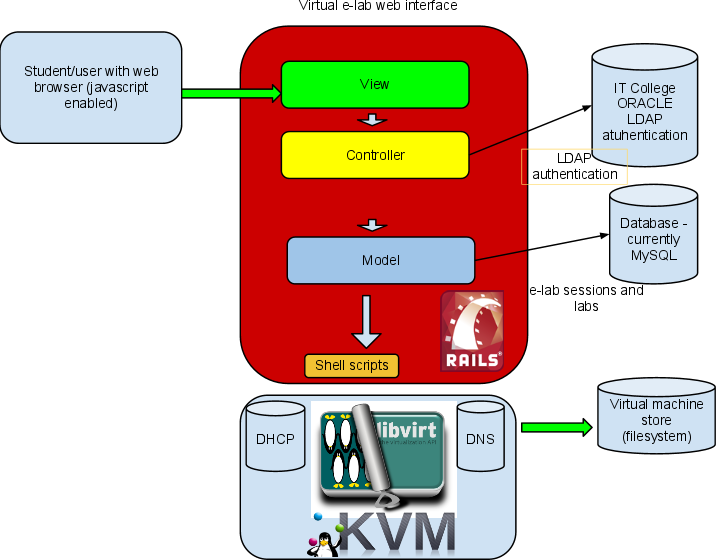
\includegraphics[width=0.8\textwidth]{architecture.png}
\caption{Architecture of Distance Laboratory}
\label{fig:Architecture of Distance Laboratory}
\end{figure}
\

\subsubsection{Security Aspects of Distance Laboratory}

\subsection{Choosing a vulnerable web application}

The main need for vulnerable web application comes from scenario: Each student installs vulnerable system and must stop basic attacks without reprogramming a web application to reflect usual system administrator's work,  install needed applications and secure them.

Although ready made virtual appliances can be used to install vulnerable web application the
system administrator should be able to install vulnerable application itself to understood a main architecture of web application to choose best protection methods. Therefore chosen application should be free and open source, easily installable, implement at leas stored and reflected \gls{XSS} and several injection type attacks like \gls{SQLi} (usual and blind) and \gls{CSRF}.

\subsubsection{WebGoat}
WebGoat is a free, open source insecure J2EE web application designed to teach web application security lessons.  However the WebGoat is one of the best application for teaching the installation and J2EE requirement is not suitable for system administrators with lesser skills even authors did installation script it hides too many steps valuable for students. 


\subsubsection{Damn Vulnerable Web Application}
The Damn Vulnerable Web Application \gls{DVWA} is web application with several vulnerabilities to be suitable for testing several security vulnerabilities and tools. However, the tool does not implement all \gls{OWASP} top ten attacks the most relevant are presented. The tool is written using PHP/MySQL which are taught for all \gls{EITC} students and known also by system administrators. Moreover the tool is designed for learning and students can choose difficulty level of exploiting \citep{website:dvwa}.

Although the progam is easy to install. Integrated study materials, variable level of  difficulties of vulnerability, the coverage is not best but sufficient.

\subsubsection{NOWASP (Mutillidae)}
NOWASP (Mutillidae) Web Pen-Test Practice Application is a free, open source vulnerable web-application for labs, security enthusiast, classrooms, \gls{CTF}, and vulnerability assessment tool targets. \citep{website:Mutillidae} Although, the tool have video, study materials, good support for \gls{OWASP} top ten the development is relied to one person and community support is thin.
\subsubsection{SQLol}
SQLol is free and open source web application designed to test \gls{SQLi} type injectons and complatible with \gls{MySQL}, gls{PostgreSQL} and uses \gls{PHP}.
cons: only supports \gls{SQLi}
pros: comprehensive  \gls{SQLi} study materials.

 This application was released at at Austin Hackers Association meeting 0x3f by Daniel “unicornFurnace” Crowley of Trustwave Holdings, Inc. – Spider Labs.
Link: https://github.com/SpiderLabs/SQLol



Because of defensive nature on developed course only simple vulnerabilities are needed to demonstrate a problem and all vulnerable applications are suitable for installing. To create diversity all applications what can installed easily can be used in lab. All examples are given using \gls{DVWA} but to get the grade every student should choose another vulnerable application, install it and protect it.

%http://pentestlab.org/10-vulnerable-web-applications-you-can-play-with/ - todo 
Practical Intrusion Analysis book - WAF võrdlus \citep{book:practica_intrusion_analysis}
\gls{CSRF}
Protection using mod\_security
\url{http://blog.spiderlabs.com/2011/01/detecting-malice-with-modsecurity-csrf-attacks.html}

\gls{XSS}
{
\color{red} *Kui avastad, kust on malicious script included siis saab esitada avalduse, et see domeen/virtualhost kinni pandaks...(see võiks olla tulevikus osa laborist.

http://www.dcortesi.com/blog/2009/04/11/twitter-stalkdaily-worm-postmortem/
}





\subsection{Testing the e-course}

\section{Implementation}

Implementation phase (train the instructor, prepare the learners (veenduda, et eeldused on korras ja nad saavad hakkama wiki ja elabiga ja virtualiseerimisega), arrange the learning space)
According to \gls{ADDIE} model...
Siin saame teada, kui palju aega kulub mingi osa peale ja kui realistlik oli plaan.

\subsection{Organizational role}

\subsection{Social role}

\subsection{Pedagogical role}
